\begin{figure}[!htb]
\begin{center}
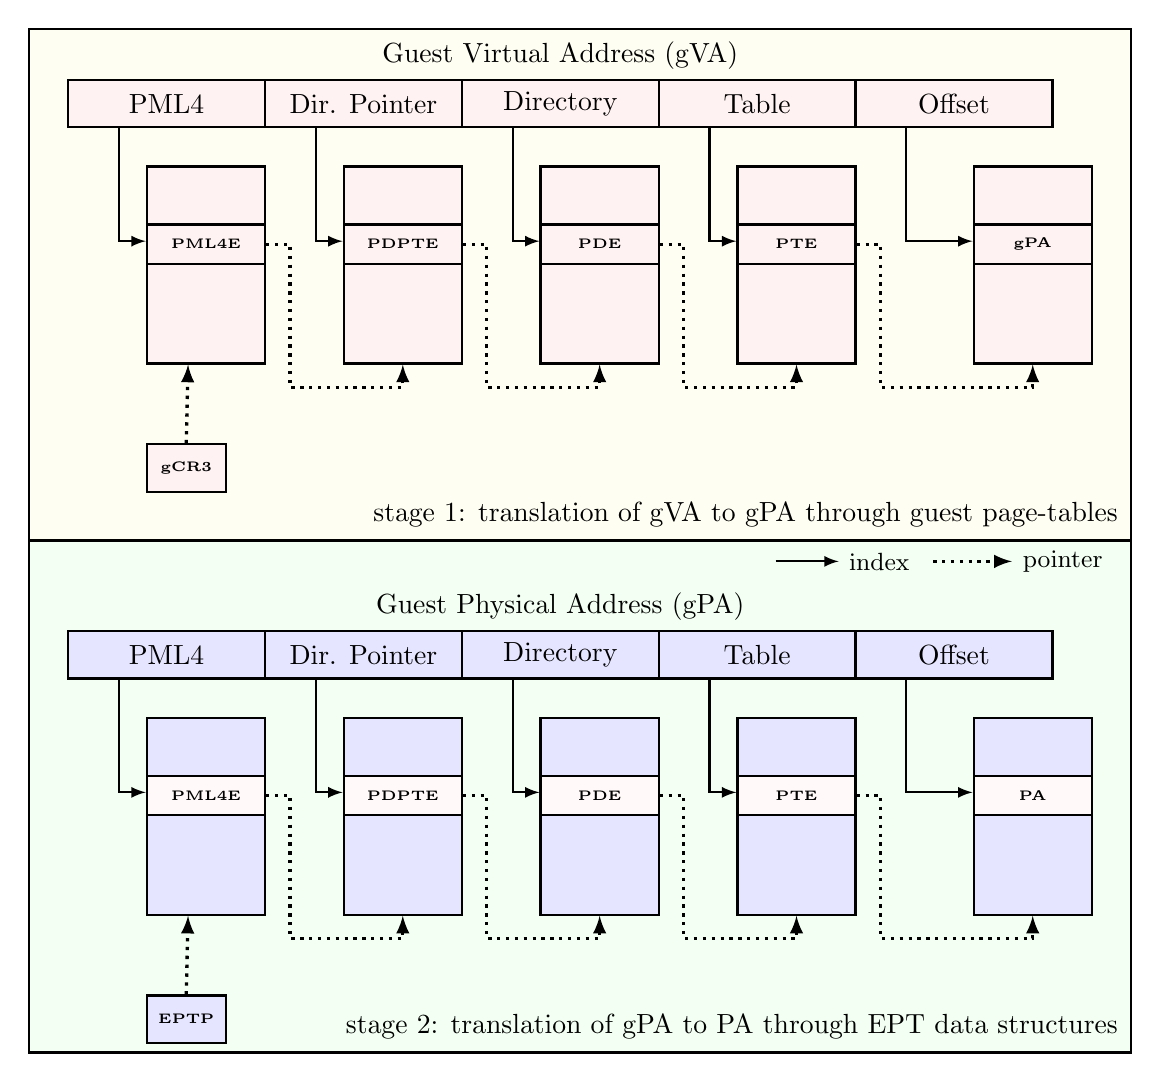
\begin{tikzpicture}

\node at (-0.5,-5-0.25) [rectangle, draw=black, thick, fill=yellow!5, minimum height = 6.5cm, minimum width = 14cm, anchor=south west] (stage1) {};
\node [above left, inner sep=5pt] at (stage1.south east) {\textbf\small{{stage 1: translation of gVA to gPA through guest page-tables}}};

\node at (0,0) [rectangle, draw=black, thick, fill=pink!20, minimum height = 0.6cm, minimum width = 2.5cm, anchor=south west] (gpml4) {PML4};
\node at (0+2.5,0) [rectangle, draw=black, thick, fill=pink!20, minimum height = 0.6cm, minimum width = 2.5cm, anchor=south west] (gdirptr) {Dir. Pointer};
\node at (0+2.5+2.5,0) [rectangle, draw=black, thick, fill=pink!20, minimum height = 0.6cm, minimum width = 2.5cm, anchor=south west] (gdir) {Directory};
\node [above, align=center] at (gdir.north) {\textbf\small{{Guest Virtual Address (gVA)}}};
\node at (0+2.5+2.5+2.5,0) [rectangle, draw=black, thick, fill=pink!20, minimum height = 0.6cm, minimum width = 2.5cm, anchor=south west] (gtbl) {Table};
\node at (0+2.5+2.5+2.5+2.5,0) [rectangle, draw=black, thick, fill=pink!20, minimum height = 0.6cm, minimum width = 2.5cm, anchor=south west] (goff) {Offset};


\node at (1.0,-3) [rectangle, draw=black, thick, fill=pink!20, minimum height = 2.5cm, minimum width = 1.5cm, anchor=south west] (gpgpml4) {};
\node [rectangle, draw=black, thick, fill=pink!20, minimum height = 0.5cm, minimum width = 1.5cm, anchor=south west] at (gpgpml4.west) (gpgpml4e) 
				{\tiny\textbf{{PML4E}}};

\node at (1.0,-4)  [rectangle, draw=black, thick, fill=pink!20, minimum height = 0.6cm, minimum width = 1.0cm, anchor=north west] (gcr3) 
				{\tiny\textbf{{gCR3}}};

\node at (3.5,-3) [rectangle, draw=black, thick, fill=pink!20, minimum height = 2.5cm, minimum width = 1.5cm, anchor=south west] (gpgdirptr) {};
\node [rectangle, draw=black, thick, fill=pink!20, minimum height = 0.5cm, minimum width = 1.5cm, anchor=south west] at (gpgdirptr.west) 
			    (gpgdirptre) {\tiny\textbf{{PDPTE}}};
\node at (6,-3) [rectangle, draw=black, thick, fill=pink!20, minimum height = 2.5cm, minimum width = 1.5cm, anchor=south west] (gpgdir) {};
\node [rectangle, draw=black, thick, fill=pink!20, minimum height = 0.5cm, minimum width = 1.5cm, anchor=south west] at (gpgdir.west) 
                (gpgdire) {\tiny\textbf{{PDE}}};
\node at (8.5,-3) [rectangle, draw=black, thick, fill=pink!20, minimum height = 2.5cm, minimum width = 1.5cm, anchor=south west] (gpgtbl) {};
\node [rectangle, draw=black, thick, fill=pink!20, minimum height = 0.5cm, minimum width = 1.5cm, anchor=south west] at (gpgtbl.west) 
                (gpgtble) {\tiny\textbf{{PTE}}};
\node at (11.5,-3) [rectangle, draw=black, thick, fill=pink!20, minimum height = 2.5cm, minimum width = 1.5cm, anchor=south west] (gpgoff) {};
\node [rectangle, draw=black, thick, fill=pink!20, minimum height = 0.5cm, minimum width = 1.5cm, anchor=south west] at (gpgoff.west) 
                {\tiny\textbf{{gPA}}};


\begin{scope}[>=latex]	
	\draw [thick, ->] ([xshift=-4ex]gpml4.south) |- ([yshift=2ex]gpgpml4.west);
	\draw [thick, ->] ([xshift=-4ex]gdirptr.south) |- ([yshift=2ex]gpgdirptr.west);
	\draw [thick, ->] ([xshift=-4ex]gdir.south) |- ([yshift=2ex]gpgdir.west);
	\draw [thick, ->] ([xshift=-4ex]gtbl.south) |- ([yshift=2ex]gpgtbl.west);
	\draw [thick, ->] ([xshift=-4ex]goff.south) |- ([yshift=2ex]gpgoff.west);

	%\draw [thick, dotted, ->] ([yshift=-1ex]gpgpml4e.south) to [bend right=75] (gpgdirptr.south);

	\draw [very thick, dotted, ->] (gcr3.north) -- ([xshift=-1.5ex]gpgpml4.south);
	\draw [very thick, dotted, ->] (gpgpml4e.east) -| ([xshift=2ex]gpgpml4e.east) -- ([xshift=2ex, yshift=-12ex]gpgpml4e.east) -| (gpgdirptr.south);
	\draw [very thick, dotted, ->] (gpgdirptre.east) -| ([xshift=2ex]gpgdirptre.east) -- ([xshift=2ex, yshift=-12ex]gpgdirptre.east) -| (gpgdir.south);
	\draw [very thick, dotted, ->] (gpgdire.east) -| ([xshift=2ex]gpgdire.east) -- ([xshift=2ex, yshift=-12ex]gpgdire.east) -| (gpgtbl.south);
	\draw [very thick, dotted, ->] (gpgtble.east) -| ([xshift=2ex]gpgtble.east) -- ([xshift=2ex, yshift=-12ex]gpgtble.east) -| (gpgoff.south);	

\end{scope}

\node at (-0.5,-5-7+0.25) [rectangle, draw=black, thick, fill=green!5, minimum height = 6.5cm, minimum width = 14cm, anchor=south west] (stage2) {};
\node [above left, inner sep=5pt] at (stage2.south east) {\textbf\small{{stage 2: translation of gPA to PA through EPT data structures}}};

\node at (0,0-7) [rectangle, draw=black, thick, fill=blue!10, minimum height = 0.6cm, minimum width = 2.5cm, anchor=south west] (gpml4) {PML4};
\node at (0+2.5,0-7) [rectangle, draw=black, thick, fill=blue!10, minimum height = 0.6cm, minimum width = 2.5cm, anchor=south west] (gdirptr) {Dir. Pointer};
\node at (0+2.5+2.5,0-7) [rectangle, draw=black, thick, fill=blue!10, minimum height = 0.6cm, minimum width = 2.5cm, anchor=south west] (gdir) {Directory};
\node [above, align=center] at (gdir.north) {\textbf\small{{Guest Physical Address (gPA)}}};
\node at (0+2.5+2.5+2.5,0-7) [rectangle, draw=black, thick, fill=blue!10, minimum height = 0.6cm, minimum width = 2.5cm, anchor=south west] (gtbl) {Table};
\node at (0+2.5+2.5+2.5+2.5,0-7) [rectangle, draw=black, thick, fill=blue!10, minimum height = 0.6cm, minimum width = 2.5cm, anchor=south west] (goff) {Offset};


\node at (1.0,-3-7) [rectangle, draw=black, thick, fill=blue!10, minimum height = 2.5cm, minimum width = 1.5cm, anchor=south west] (gpgpml4) {};
\node [rectangle, draw=black, thick, fill=pink!10, minimum height = 0.5cm, minimum width = 1.5cm, anchor=south west] at (gpgpml4.west) (gpgpml4e) 
				{\tiny\textbf{{PML4E}}};

\node at (1.0,-4-7)  [rectangle, draw=black, thick, fill=blue!10, minimum height = 0.6cm, minimum width = 1.0cm, anchor=north west] (eptp) 
				{\tiny\textbf{{EPTP}}};

\node at (3.5,-3-7) [rectangle, draw=black, thick, fill=blue!10, minimum height = 2.5cm, minimum width = 1.5cm, anchor=south west] (gpgdirptr) {};
\node [rectangle, draw=black, thick, fill=pink!10, minimum height = 0.5cm, minimum width = 1.5cm, anchor=south west] at (gpgdirptr.west) 
			    (gpgdirptre) {\tiny\textbf{{PDPTE}}};
\node at (6,-3-7) [rectangle, draw=black, thick, fill=blue!10, minimum height = 2.5cm, minimum width = 1.5cm, anchor=south west] (gpgdir) {};
\node [rectangle, draw=black, thick, fill=pink!10, minimum height = 0.5cm, minimum width = 1.5cm, anchor=south west] at (gpgdir.west) 
                (gpgdire) {\tiny\textbf{{PDE}}};
\node at (8.5,-3-7) [rectangle, draw=black, thick, fill=blue!10, minimum height = 2.5cm, minimum width = 1.5cm, anchor=south west] (gpgtbl) {};
\node [rectangle, draw=black, thick, fill=pink!10, minimum height = 0.5cm, minimum width = 1.5cm, anchor=south west] at (gpgtbl.west) 
                (gpgtble) {\tiny\textbf{{PTE}}};
\node at (11.5,-3-7) [rectangle, draw=black, thick, fill=blue!10, minimum height = 2.5cm, minimum width = 1.5cm, anchor=south west] (gpgoff) {};
\node [rectangle, draw=black, thick, fill=pink!10, minimum height = 0.5cm, minimum width = 1.5cm, anchor=south west] at (gpgoff.west) 
                {\tiny\textbf{{PA}}};

\begin{scope}[>=latex]	
	\draw [thick, ->] ([xshift=-4ex]gpml4.south) |- ([yshift=2ex]gpgpml4.west);
	\draw [thick, ->] ([xshift=-4ex]gdirptr.south) |- ([yshift=2ex]gpgdirptr.west);
	\draw [thick, ->] ([xshift=-4ex]gdir.south) |- ([yshift=2ex]gpgdir.west);
	\draw [thick, ->] ([xshift=-4ex]gtbl.south) |- ([yshift=2ex]gpgtbl.west);
	\draw [thick, ->] ([xshift=-4ex]goff.south) |- ([yshift=2ex]gpgoff.west);

	\draw [very thick, dotted, ->] (eptp.north) -- ([xshift=-1.5ex]gpgpml4.south);
	\draw [very thick, dotted, ->] (gpgpml4e.east) -| ([xshift=2ex]gpgpml4e.east) -- ([xshift=2ex, yshift=-12ex]gpgpml4e.east) -| (gpgdirptr.south);
	\draw [very thick, dotted, ->] (gpgdirptre.east) -| ([xshift=2ex]gpgdirptre.east) -- ([xshift=2ex, yshift=-12ex]gpgdirptre.east) -| (gpgdir.south);
	\draw [very thick, dotted, ->] (gpgdire.east) -| ([xshift=2ex]gpgdire.east) -- ([xshift=2ex, yshift=-12ex]gpgdire.east) -| (gpgtbl.south);
	\draw [very thick, dotted, ->] (gpgtble.east) -| ([xshift=2ex]gpgtble.east) -- ([xshift=2ex, yshift=-12ex]gpgtble.east) -| (gpgoff.south);	

	\draw [very thick, dotted, ->] (11,-5.5) -- (12, -5.5) node [right] {\small{pointer}};
	\draw [thick, ->] (9,-5.5) -- (9.8, -5.5) node [right] {\small{index}};
\end{scope}

\end{tikzpicture}
\end{center}
\ifreport
\caption{MMU Virtualization (inspired from \cite{West:2016:VSK:2966277.2935748})}
\fi
\label{fig-vmmu}
\end{figure}
